% Created by tikzDevice version 0.11 on 2018-03-29 23:08:52
% !TEX encoding = UTF-8 Unicode
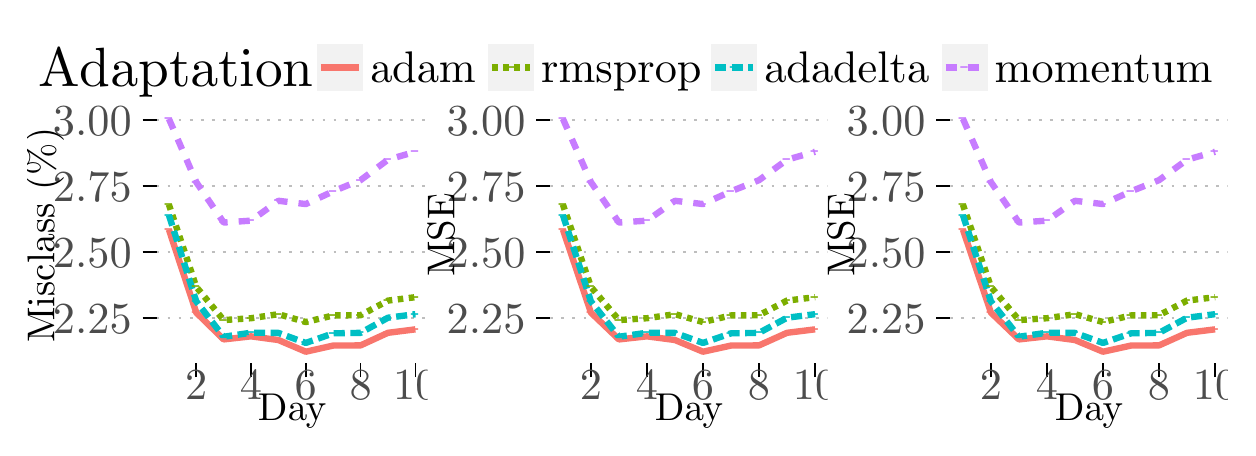
\begin{tikzpicture}[x=1pt,y=1pt]
\definecolor{fillColor}{RGB}{255,255,255}
\path[use as bounding box,fill=fillColor,fill opacity=0.00] (0,0) rectangle (433.62,144.54);
\begin{scope}
\path[clip] (  0.00,  0.00) rectangle (433.62,144.54);
\definecolor{fillColor}{RGB}{255,255,255}

\path[fill=fillColor] ( -1.83,115.81) rectangle (435.45,144.54);
\end{scope}
\begin{scope}
\path[clip] (  0.00,  0.00) rectangle (433.62,144.54);
\definecolor{drawColor}{RGB}{0,0,0}

\node[text=drawColor,anchor=base west,inner sep=0pt, outer sep=0pt, scale=  2.00] at (  3.86,123.29) {Adaptation};
\end{scope}
\begin{scope}
\path[clip] (  0.00,  0.00) rectangle (433.62,144.54);
\definecolor{drawColor}{RGB}{255,255,255}
\definecolor{fillColor}{gray}{0.95}

\path[draw=drawColor,line width= 0.6pt,line join=round,line cap=round,fill=fillColor] (104.19,121.50) rectangle (121.53,138.85);
\end{scope}
\begin{scope}
\path[clip] (  0.00,  0.00) rectangle (433.62,144.54);
\definecolor{drawColor}{RGB}{248,118,109}

\path[draw=drawColor,line width= 2.3pt,line join=round] (105.92,130.18) -- (119.80,130.18);
\end{scope}
\begin{scope}
\path[clip] (  0.00,  0.00) rectangle (433.62,144.54);
\definecolor{drawColor}{RGB}{248,118,109}

\node[text=drawColor,anchor=base,inner sep=0pt, outer sep=0pt, scale=  1.00] at (112.86,128.01) {-};
\end{scope}
\begin{scope}
\path[clip] (  0.00,  0.00) rectangle (433.62,144.54);
\definecolor{drawColor}{RGB}{255,255,255}
\definecolor{fillColor}{gray}{0.95}

\path[draw=drawColor,line width= 0.6pt,line join=round,line cap=round,fill=fillColor] (166.04,121.50) rectangle (183.39,138.85);
\end{scope}
\begin{scope}
\path[clip] (  0.00,  0.00) rectangle (433.62,144.54);
\definecolor{drawColor}{RGB}{124,174,0}

\path[draw=drawColor,line width= 2.3pt,dash pattern=on 2pt off 2pt ,line join=round] (167.78,130.18) -- (181.65,130.18);
\end{scope}
\begin{scope}
\path[clip] (  0.00,  0.00) rectangle (433.62,144.54);
\definecolor{drawColor}{RGB}{124,174,0}

\node[text=drawColor,anchor=base,inner sep=0pt, outer sep=0pt, scale=  1.00] at (174.71,128.01) {-};
\end{scope}
\begin{scope}
\path[clip] (  0.00,  0.00) rectangle (433.62,144.54);
\definecolor{drawColor}{RGB}{255,255,255}
\definecolor{fillColor}{gray}{0.95}

\path[draw=drawColor,line width= 0.6pt,line join=round,line cap=round,fill=fillColor] (246.62,121.50) rectangle (263.97,138.85);
\end{scope}
\begin{scope}
\path[clip] (  0.00,  0.00) rectangle (433.62,144.54);
\definecolor{drawColor}{RGB}{0,191,196}

\path[draw=drawColor,line width= 2.3pt,dash pattern=on 4pt off 2pt ,line join=round] (248.36,130.18) -- (262.23,130.18);
\end{scope}
\begin{scope}
\path[clip] (  0.00,  0.00) rectangle (433.62,144.54);
\definecolor{drawColor}{RGB}{0,191,196}

\node[text=drawColor,anchor=base,inner sep=0pt, outer sep=0pt, scale=  1.00] at (255.30,128.01) {-};
\end{scope}
\begin{scope}
\path[clip] (  0.00,  0.00) rectangle (433.62,144.54);
\definecolor{drawColor}{RGB}{255,255,255}
\definecolor{fillColor}{gray}{0.95}

\path[draw=drawColor,line width= 0.6pt,line join=round,line cap=round,fill=fillColor] (329.93,121.50) rectangle (347.27,138.85);
\end{scope}
\begin{scope}
\path[clip] (  0.00,  0.00) rectangle (433.62,144.54);
\definecolor{drawColor}{RGB}{199,124,255}

\path[draw=drawColor,line width= 2.3pt,dash pattern=on 4pt off 4pt ,line join=round] (331.66,130.18) -- (345.54,130.18);
\end{scope}
\begin{scope}
\path[clip] (  0.00,  0.00) rectangle (433.62,144.54);
\definecolor{drawColor}{RGB}{199,124,255}

\node[text=drawColor,anchor=base,inner sep=0pt, outer sep=0pt, scale=  1.00] at (338.60,128.01) {-};
\end{scope}
\begin{scope}
\path[clip] (  0.00,  0.00) rectangle (433.62,144.54);
\definecolor{drawColor}{RGB}{0,0,0}

\node[text=drawColor,anchor=base west,inner sep=0pt, outer sep=0pt, scale=  1.60] at (123.70,124.67) {adam};
\end{scope}
\begin{scope}
\path[clip] (  0.00,  0.00) rectangle (433.62,144.54);
\definecolor{drawColor}{RGB}{0,0,0}

\node[text=drawColor,anchor=base west,inner sep=0pt, outer sep=0pt, scale=  1.60] at (185.56,124.67) {rmsprop};
\end{scope}
\begin{scope}
\path[clip] (  0.00,  0.00) rectangle (433.62,144.54);
\definecolor{drawColor}{RGB}{0,0,0}

\node[text=drawColor,anchor=base west,inner sep=0pt, outer sep=0pt, scale=  1.60] at (266.14,124.67) {adadelta};
\end{scope}
\begin{scope}
\path[clip] (  0.00,  0.00) rectangle (433.62,144.54);
\definecolor{drawColor}{RGB}{0,0,0}

\node[text=drawColor,anchor=base west,inner sep=0pt, outer sep=0pt, scale=  1.60] at (349.44,124.67) {momentum};
\end{scope}
\begin{scope}
\path[clip] (  0.00,  0.00) rectangle (144.54,115.81);
\definecolor{drawColor}{RGB}{255,255,255}
\definecolor{fillColor}{RGB}{255,255,255}

\path[draw=drawColor,line width= 0.6pt,line join=round,line cap=round,fill=fillColor] (  0.00,  0.00) rectangle (144.54,115.81);
\end{scope}
\begin{scope}
\path[clip] ( 46.57, 23.24) rectangle (144.54,115.81);
\definecolor{fillColor}{RGB}{255,255,255}

\path[fill=fillColor] ( 46.57, 23.24) rectangle (144.54,115.81);
\definecolor{drawColor}{RGB}{255,255,255}

\path[draw=drawColor,line width= 0.3pt,line join=round] ( 46.57, 27.76) --
	(144.54, 27.76);

\path[draw=drawColor,line width= 0.3pt,line join=round] ( 46.57, 51.58) --
	(144.54, 51.58);

\path[draw=drawColor,line width= 0.3pt,line join=round] ( 46.57, 75.40) --
	(144.54, 75.40);

\path[draw=drawColor,line width= 0.3pt,line join=round] ( 46.57, 99.22) --
	(144.54, 99.22);

\path[draw=drawColor,line width= 0.3pt,line join=round] ( 51.03, 23.24) --
	( 51.03,115.81);

\path[draw=drawColor,line width= 0.3pt,line join=round] ( 70.82, 23.24) --
	( 70.82,115.81);

\path[draw=drawColor,line width= 0.3pt,line join=round] ( 90.61, 23.24) --
	( 90.61,115.81);

\path[draw=drawColor,line width= 0.3pt,line join=round] (110.40, 23.24) --
	(110.40,115.81);

\path[draw=drawColor,line width= 0.3pt,line join=round] (130.19, 23.24) --
	(130.19,115.81);
\definecolor{drawColor}{RGB}{190,190,190}

\path[draw=drawColor,line width= 0.6pt,dash pattern=on 1pt off 3pt ,line join=round] ( 46.57, 39.67) --
	(144.54, 39.67);

\path[draw=drawColor,line width= 0.6pt,dash pattern=on 1pt off 3pt ,line join=round] ( 46.57, 63.49) --
	(144.54, 63.49);

\path[draw=drawColor,line width= 0.6pt,dash pattern=on 1pt off 3pt ,line join=round] ( 46.57, 87.31) --
	(144.54, 87.31);

\path[draw=drawColor,line width= 0.6pt,dash pattern=on 1pt off 3pt ,line join=round] ( 46.57,111.13) --
	(144.54,111.13);
\definecolor{drawColor}{RGB}{255,255,255}

\path[draw=drawColor,line width= 0.6pt,line join=round] ( 60.92, 23.24) --
	( 60.92,115.81);

\path[draw=drawColor,line width= 0.6pt,line join=round] ( 80.71, 23.24) --
	( 80.71,115.81);

\path[draw=drawColor,line width= 0.6pt,line join=round] (100.50, 23.24) --
	(100.50,115.81);

\path[draw=drawColor,line width= 0.6pt,line join=round] (120.30, 23.24) --
	(120.30,115.81);

\path[draw=drawColor,line width= 0.6pt,line join=round] (140.09, 23.24) --
	(140.09,115.81);
\definecolor{drawColor}{RGB}{248,118,109}

\path[draw=drawColor,line width= 2.3pt,line join=round] ( 51.03, 71.59) --
	( 60.92, 41.58) --
	( 70.82, 31.89) --
	( 80.71, 33.00) --
	( 90.61, 31.67) --
	(100.50, 27.45) --
	(110.40, 29.67) --
	(120.30, 29.73) --
	(130.19, 34.28) --
	(140.09, 35.53);
\definecolor{drawColor}{RGB}{124,174,0}

\path[draw=drawColor,line width= 2.3pt,dash pattern=on 2pt off 2pt ,line join=round] ( 51.03, 80.64) --
	( 60.92, 50.87) --
	( 70.82, 38.88) --
	( 80.71, 39.55) --
	( 90.61, 41.01) --
	(100.50, 38.17) --
	(110.40, 40.56) --
	(120.30, 40.63) --
	(130.19, 45.92) --
	(140.09, 47.15);
\definecolor{drawColor}{RGB}{0,191,196}

\path[draw=drawColor,line width= 2.3pt,dash pattern=on 4pt off 2pt ,line join=round] ( 51.03, 76.83) --
	( 60.92, 45.63) --
	( 70.82, 32.85) --
	( 80.71, 34.31) --
	( 90.61, 34.24) --
	(100.50, 30.62) --
	(110.40, 34.09) --
	(120.30, 34.26) --
	(130.19, 39.73) --
	(140.09, 41.01);
\definecolor{drawColor}{RGB}{199,124,255}

\path[draw=drawColor,line width= 2.3pt,dash pattern=on 4pt off 4pt ,line join=round] ( 51.03,111.61) --
	( 60.92, 88.74) --
	( 70.82, 74.13) --
	( 80.71, 74.81) --
	( 90.61, 81.98) --
	(100.50, 80.80) --
	(110.40, 85.41) --
	(120.30, 89.45) --
	(130.19, 96.84) --
	(140.09, 99.70);
\definecolor{drawColor}{RGB}{248,118,109}

\node[text=drawColor,anchor=base,inner sep=0pt, outer sep=0pt, scale=  1.00] at ( 51.03, 69.43) {-};

\node[text=drawColor,anchor=base,inner sep=0pt, outer sep=0pt, scale=  1.00] at ( 60.92, 39.42) {-};

\node[text=drawColor,anchor=base,inner sep=0pt, outer sep=0pt, scale=  1.00] at ( 70.82, 29.73) {-};

\node[text=drawColor,anchor=base,inner sep=0pt, outer sep=0pt, scale=  1.00] at ( 80.71, 30.84) {-};

\node[text=drawColor,anchor=base,inner sep=0pt, outer sep=0pt, scale=  1.00] at ( 90.61, 29.51) {-};

\node[text=drawColor,anchor=base,inner sep=0pt, outer sep=0pt, scale=  1.00] at (100.50, 25.28) {-};

\node[text=drawColor,anchor=base,inner sep=0pt, outer sep=0pt, scale=  1.00] at (110.40, 27.51) {-};

\node[text=drawColor,anchor=base,inner sep=0pt, outer sep=0pt, scale=  1.00] at (120.30, 27.57) {-};

\node[text=drawColor,anchor=base,inner sep=0pt, outer sep=0pt, scale=  1.00] at (130.19, 32.11) {-};

\node[text=drawColor,anchor=base,inner sep=0pt, outer sep=0pt, scale=  1.00] at (140.09, 33.37) {-};
\definecolor{drawColor}{RGB}{124,174,0}

\node[text=drawColor,anchor=base,inner sep=0pt, outer sep=0pt, scale=  1.00] at ( 51.03, 78.48) {-};

\node[text=drawColor,anchor=base,inner sep=0pt, outer sep=0pt, scale=  1.00] at ( 60.92, 48.71) {-};

\node[text=drawColor,anchor=base,inner sep=0pt, outer sep=0pt, scale=  1.00] at ( 70.82, 36.72) {-};

\node[text=drawColor,anchor=base,inner sep=0pt, outer sep=0pt, scale=  1.00] at ( 80.71, 37.39) {-};

\node[text=drawColor,anchor=base,inner sep=0pt, outer sep=0pt, scale=  1.00] at ( 90.61, 38.84) {-};

\node[text=drawColor,anchor=base,inner sep=0pt, outer sep=0pt, scale=  1.00] at (100.50, 36.00) {-};

\node[text=drawColor,anchor=base,inner sep=0pt, outer sep=0pt, scale=  1.00] at (110.40, 38.40) {-};

\node[text=drawColor,anchor=base,inner sep=0pt, outer sep=0pt, scale=  1.00] at (120.30, 38.46) {-};

\node[text=drawColor,anchor=base,inner sep=0pt, outer sep=0pt, scale=  1.00] at (130.19, 43.76) {-};

\node[text=drawColor,anchor=base,inner sep=0pt, outer sep=0pt, scale=  1.00] at (140.09, 44.99) {-};
\definecolor{drawColor}{RGB}{0,191,196}

\node[text=drawColor,anchor=base,inner sep=0pt, outer sep=0pt, scale=  1.00] at ( 51.03, 74.67) {-};

\node[text=drawColor,anchor=base,inner sep=0pt, outer sep=0pt, scale=  1.00] at ( 60.92, 43.47) {-};

\node[text=drawColor,anchor=base,inner sep=0pt, outer sep=0pt, scale=  1.00] at ( 70.82, 30.68) {-};

\node[text=drawColor,anchor=base,inner sep=0pt, outer sep=0pt, scale=  1.00] at ( 80.71, 32.15) {-};

\node[text=drawColor,anchor=base,inner sep=0pt, outer sep=0pt, scale=  1.00] at ( 90.61, 32.08) {-};

\node[text=drawColor,anchor=base,inner sep=0pt, outer sep=0pt, scale=  1.00] at (100.50, 28.46) {-};

\node[text=drawColor,anchor=base,inner sep=0pt, outer sep=0pt, scale=  1.00] at (110.40, 31.93) {-};

\node[text=drawColor,anchor=base,inner sep=0pt, outer sep=0pt, scale=  1.00] at (120.30, 32.09) {-};

\node[text=drawColor,anchor=base,inner sep=0pt, outer sep=0pt, scale=  1.00] at (130.19, 37.56) {-};

\node[text=drawColor,anchor=base,inner sep=0pt, outer sep=0pt, scale=  1.00] at (140.09, 38.84) {-};
\definecolor{drawColor}{RGB}{199,124,255}

\node[text=drawColor,anchor=base,inner sep=0pt, outer sep=0pt, scale=  1.00] at ( 51.03,109.44) {-};

\node[text=drawColor,anchor=base,inner sep=0pt, outer sep=0pt, scale=  1.00] at ( 60.92, 86.58) {-};

\node[text=drawColor,anchor=base,inner sep=0pt, outer sep=0pt, scale=  1.00] at ( 70.82, 71.97) {-};

\node[text=drawColor,anchor=base,inner sep=0pt, outer sep=0pt, scale=  1.00] at ( 80.71, 72.64) {-};

\node[text=drawColor,anchor=base,inner sep=0pt, outer sep=0pt, scale=  1.00] at ( 90.61, 79.81) {-};

\node[text=drawColor,anchor=base,inner sep=0pt, outer sep=0pt, scale=  1.00] at (100.50, 78.64) {-};

\node[text=drawColor,anchor=base,inner sep=0pt, outer sep=0pt, scale=  1.00] at (110.40, 83.24) {-};

\node[text=drawColor,anchor=base,inner sep=0pt, outer sep=0pt, scale=  1.00] at (120.30, 87.29) {-};

\node[text=drawColor,anchor=base,inner sep=0pt, outer sep=0pt, scale=  1.00] at (130.19, 94.68) {-};

\node[text=drawColor,anchor=base,inner sep=0pt, outer sep=0pt, scale=  1.00] at (140.09, 97.53) {-};
\end{scope}
\begin{scope}
\path[clip] (  0.00,  0.00) rectangle (433.62,144.54);
\definecolor{drawColor}{gray}{0.30}

\node[text=drawColor,anchor=base east,inner sep=0pt, outer sep=0pt, scale=  1.60] at ( 37.57, 34.16) {2.25};

\node[text=drawColor,anchor=base east,inner sep=0pt, outer sep=0pt, scale=  1.60] at ( 37.57, 57.98) {2.50};

\node[text=drawColor,anchor=base east,inner sep=0pt, outer sep=0pt, scale=  1.60] at ( 37.57, 81.80) {2.75};

\node[text=drawColor,anchor=base east,inner sep=0pt, outer sep=0pt, scale=  1.60] at ( 37.57,105.62) {3.00};
\end{scope}
\begin{scope}
\path[clip] (  0.00,  0.00) rectangle (433.62,144.54);
\definecolor{drawColor}{RGB}{0,0,0}

\path[draw=drawColor,line width= 0.6pt,line join=round] ( 41.57, 39.67) --
	( 46.57, 39.67);

\path[draw=drawColor,line width= 0.6pt,line join=round] ( 41.57, 63.49) --
	( 46.57, 63.49);

\path[draw=drawColor,line width= 0.6pt,line join=round] ( 41.57, 87.31) --
	( 46.57, 87.31);

\path[draw=drawColor,line width= 0.6pt,line join=round] ( 41.57,111.13) --
	( 46.57,111.13);
\end{scope}
\begin{scope}
\path[clip] (  0.00,  0.00) rectangle (433.62,144.54);
\definecolor{drawColor}{RGB}{0,0,0}

\path[draw=drawColor,line width= 0.6pt,line join=round] ( 60.92, 18.24) --
	( 60.92, 23.24);

\path[draw=drawColor,line width= 0.6pt,line join=round] ( 80.71, 18.24) --
	( 80.71, 23.24);

\path[draw=drawColor,line width= 0.6pt,line join=round] (100.50, 18.24) --
	(100.50, 23.24);

\path[draw=drawColor,line width= 0.6pt,line join=round] (120.30, 18.24) --
	(120.30, 23.24);

\path[draw=drawColor,line width= 0.6pt,line join=round] (140.09, 18.24) --
	(140.09, 23.24);
\end{scope}
\begin{scope}
\path[clip] (  0.00,  0.00) rectangle (433.62,144.54);
\definecolor{drawColor}{gray}{0.30}

\node[text=drawColor,anchor=base,inner sep=0pt, outer sep=0pt, scale=  1.60] at ( 60.92, 10.22) {2};

\node[text=drawColor,anchor=base,inner sep=0pt, outer sep=0pt, scale=  1.60] at ( 80.71, 10.22) {4};

\node[text=drawColor,anchor=base,inner sep=0pt, outer sep=0pt, scale=  1.60] at (100.50, 10.22) {6};

\node[text=drawColor,anchor=base,inner sep=0pt, outer sep=0pt, scale=  1.60] at (120.30, 10.22) {8};

\node[text=drawColor,anchor=base,inner sep=0pt, outer sep=0pt, scale=  1.60] at (140.09, 10.22) {10};
\end{scope}
\begin{scope}
\path[clip] (  0.00,  0.00) rectangle (433.62,144.54);
\definecolor{drawColor}{RGB}{0,0,0}

\node[text=drawColor,anchor=base,inner sep=0pt, outer sep=0pt, scale=  1.40] at ( 95.56,  2.58) {Day};
\end{scope}
\begin{scope}
\path[clip] (  0.00,  0.00) rectangle (433.62,144.54);
\definecolor{drawColor}{RGB}{0,0,0}

\node[text=drawColor,rotate= 90.00,anchor=base,inner sep=0pt, outer sep=0pt, scale=  1.40] at (  9.64, 69.53) {Misclass (\%)};
\end{scope}
\begin{scope}
\path[clip] (144.54,  0.00) rectangle (289.08,115.81);
\definecolor{drawColor}{RGB}{255,255,255}
\definecolor{fillColor}{RGB}{255,255,255}

\path[draw=drawColor,line width= 0.6pt,line join=round,line cap=round,fill=fillColor] (144.54,  0.00) rectangle (289.08,115.81);
\end{scope}
\begin{scope}
\path[clip] (188.85, 23.24) rectangle (289.08,115.81);
\definecolor{fillColor}{RGB}{255,255,255}

\path[fill=fillColor] (188.85, 23.24) rectangle (289.08,115.81);
\definecolor{drawColor}{RGB}{255,255,255}

\path[draw=drawColor,line width= 0.3pt,line join=round] (188.85, 27.76) --
	(289.08, 27.76);

\path[draw=drawColor,line width= 0.3pt,line join=round] (188.85, 51.58) --
	(289.08, 51.58);

\path[draw=drawColor,line width= 0.3pt,line join=round] (188.85, 75.40) --
	(289.08, 75.40);

\path[draw=drawColor,line width= 0.3pt,line join=round] (188.85, 99.22) --
	(289.08, 99.22);

\path[draw=drawColor,line width= 0.3pt,line join=round] (193.40, 23.24) --
	(193.40,115.81);

\path[draw=drawColor,line width= 0.3pt,line join=round] (213.65, 23.24) --
	(213.65,115.81);

\path[draw=drawColor,line width= 0.3pt,line join=round] (233.90, 23.24) --
	(233.90,115.81);

\path[draw=drawColor,line width= 0.3pt,line join=round] (254.15, 23.24) --
	(254.15,115.81);

\path[draw=drawColor,line width= 0.3pt,line join=round] (274.40, 23.24) --
	(274.40,115.81);
\definecolor{drawColor}{RGB}{190,190,190}

\path[draw=drawColor,line width= 0.6pt,dash pattern=on 1pt off 3pt ,line join=round] (188.85, 39.67) --
	(289.08, 39.67);

\path[draw=drawColor,line width= 0.6pt,dash pattern=on 1pt off 3pt ,line join=round] (188.85, 63.49) --
	(289.08, 63.49);

\path[draw=drawColor,line width= 0.6pt,dash pattern=on 1pt off 3pt ,line join=round] (188.85, 87.31) --
	(289.08, 87.31);

\path[draw=drawColor,line width= 0.6pt,dash pattern=on 1pt off 3pt ,line join=round] (188.85,111.13) --
	(289.08,111.13);
\definecolor{drawColor}{RGB}{255,255,255}

\path[draw=drawColor,line width= 0.6pt,line join=round] (203.53, 23.24) --
	(203.53,115.81);

\path[draw=drawColor,line width= 0.6pt,line join=round] (223.78, 23.24) --
	(223.78,115.81);

\path[draw=drawColor,line width= 0.6pt,line join=round] (244.03, 23.24) --
	(244.03,115.81);

\path[draw=drawColor,line width= 0.6pt,line join=round] (264.28, 23.24) --
	(264.28,115.81);

\path[draw=drawColor,line width= 0.6pt,line join=round] (284.52, 23.24) --
	(284.52,115.81);
\definecolor{drawColor}{RGB}{248,118,109}

\path[draw=drawColor,line width= 2.3pt,line join=round] (193.40, 71.59) --
	(203.53, 41.58) --
	(213.65, 31.89) --
	(223.78, 33.00) --
	(233.90, 31.67) --
	(244.03, 27.45) --
	(254.15, 29.67) --
	(264.28, 29.73) --
	(274.40, 34.28) --
	(284.52, 35.53);
\definecolor{drawColor}{RGB}{124,174,0}

\path[draw=drawColor,line width= 2.3pt,dash pattern=on 2pt off 2pt ,line join=round] (193.40, 80.64) --
	(203.53, 50.87) --
	(213.65, 38.88) --
	(223.78, 39.55) --
	(233.90, 41.01) --
	(244.03, 38.17) --
	(254.15, 40.56) --
	(264.28, 40.63) --
	(274.40, 45.92) --
	(284.52, 47.15);
\definecolor{drawColor}{RGB}{0,191,196}

\path[draw=drawColor,line width= 2.3pt,dash pattern=on 4pt off 2pt ,line join=round] (193.40, 76.83) --
	(203.53, 45.63) --
	(213.65, 32.85) --
	(223.78, 34.31) --
	(233.90, 34.24) --
	(244.03, 30.62) --
	(254.15, 34.09) --
	(264.28, 34.26) --
	(274.40, 39.73) --
	(284.52, 41.01);
\definecolor{drawColor}{RGB}{199,124,255}

\path[draw=drawColor,line width= 2.3pt,dash pattern=on 4pt off 4pt ,line join=round] (193.40,111.61) --
	(203.53, 88.74) --
	(213.65, 74.13) --
	(223.78, 74.81) --
	(233.90, 81.98) --
	(244.03, 80.80) --
	(254.15, 85.41) --
	(264.28, 89.45) --
	(274.40, 96.84) --
	(284.52, 99.70);
\definecolor{drawColor}{RGB}{248,118,109}

\node[text=drawColor,anchor=base,inner sep=0pt, outer sep=0pt, scale=  1.00] at (193.40, 69.43) {-};

\node[text=drawColor,anchor=base,inner sep=0pt, outer sep=0pt, scale=  1.00] at (203.53, 39.42) {-};

\node[text=drawColor,anchor=base,inner sep=0pt, outer sep=0pt, scale=  1.00] at (213.65, 29.73) {-};

\node[text=drawColor,anchor=base,inner sep=0pt, outer sep=0pt, scale=  1.00] at (223.78, 30.84) {-};

\node[text=drawColor,anchor=base,inner sep=0pt, outer sep=0pt, scale=  1.00] at (233.90, 29.51) {-};

\node[text=drawColor,anchor=base,inner sep=0pt, outer sep=0pt, scale=  1.00] at (244.03, 25.28) {-};

\node[text=drawColor,anchor=base,inner sep=0pt, outer sep=0pt, scale=  1.00] at (254.15, 27.51) {-};

\node[text=drawColor,anchor=base,inner sep=0pt, outer sep=0pt, scale=  1.00] at (264.28, 27.57) {-};

\node[text=drawColor,anchor=base,inner sep=0pt, outer sep=0pt, scale=  1.00] at (274.40, 32.11) {-};

\node[text=drawColor,anchor=base,inner sep=0pt, outer sep=0pt, scale=  1.00] at (284.52, 33.37) {-};
\definecolor{drawColor}{RGB}{124,174,0}

\node[text=drawColor,anchor=base,inner sep=0pt, outer sep=0pt, scale=  1.00] at (193.40, 78.48) {-};

\node[text=drawColor,anchor=base,inner sep=0pt, outer sep=0pt, scale=  1.00] at (203.53, 48.71) {-};

\node[text=drawColor,anchor=base,inner sep=0pt, outer sep=0pt, scale=  1.00] at (213.65, 36.72) {-};

\node[text=drawColor,anchor=base,inner sep=0pt, outer sep=0pt, scale=  1.00] at (223.78, 37.39) {-};

\node[text=drawColor,anchor=base,inner sep=0pt, outer sep=0pt, scale=  1.00] at (233.90, 38.84) {-};

\node[text=drawColor,anchor=base,inner sep=0pt, outer sep=0pt, scale=  1.00] at (244.03, 36.00) {-};

\node[text=drawColor,anchor=base,inner sep=0pt, outer sep=0pt, scale=  1.00] at (254.15, 38.40) {-};

\node[text=drawColor,anchor=base,inner sep=0pt, outer sep=0pt, scale=  1.00] at (264.28, 38.46) {-};

\node[text=drawColor,anchor=base,inner sep=0pt, outer sep=0pt, scale=  1.00] at (274.40, 43.76) {-};

\node[text=drawColor,anchor=base,inner sep=0pt, outer sep=0pt, scale=  1.00] at (284.52, 44.99) {-};
\definecolor{drawColor}{RGB}{0,191,196}

\node[text=drawColor,anchor=base,inner sep=0pt, outer sep=0pt, scale=  1.00] at (193.40, 74.67) {-};

\node[text=drawColor,anchor=base,inner sep=0pt, outer sep=0pt, scale=  1.00] at (203.53, 43.47) {-};

\node[text=drawColor,anchor=base,inner sep=0pt, outer sep=0pt, scale=  1.00] at (213.65, 30.68) {-};

\node[text=drawColor,anchor=base,inner sep=0pt, outer sep=0pt, scale=  1.00] at (223.78, 32.15) {-};

\node[text=drawColor,anchor=base,inner sep=0pt, outer sep=0pt, scale=  1.00] at (233.90, 32.08) {-};

\node[text=drawColor,anchor=base,inner sep=0pt, outer sep=0pt, scale=  1.00] at (244.03, 28.46) {-};

\node[text=drawColor,anchor=base,inner sep=0pt, outer sep=0pt, scale=  1.00] at (254.15, 31.93) {-};

\node[text=drawColor,anchor=base,inner sep=0pt, outer sep=0pt, scale=  1.00] at (264.28, 32.09) {-};

\node[text=drawColor,anchor=base,inner sep=0pt, outer sep=0pt, scale=  1.00] at (274.40, 37.56) {-};

\node[text=drawColor,anchor=base,inner sep=0pt, outer sep=0pt, scale=  1.00] at (284.52, 38.84) {-};
\definecolor{drawColor}{RGB}{199,124,255}

\node[text=drawColor,anchor=base,inner sep=0pt, outer sep=0pt, scale=  1.00] at (193.40,109.44) {-};

\node[text=drawColor,anchor=base,inner sep=0pt, outer sep=0pt, scale=  1.00] at (203.53, 86.58) {-};

\node[text=drawColor,anchor=base,inner sep=0pt, outer sep=0pt, scale=  1.00] at (213.65, 71.97) {-};

\node[text=drawColor,anchor=base,inner sep=0pt, outer sep=0pt, scale=  1.00] at (223.78, 72.64) {-};

\node[text=drawColor,anchor=base,inner sep=0pt, outer sep=0pt, scale=  1.00] at (233.90, 79.81) {-};

\node[text=drawColor,anchor=base,inner sep=0pt, outer sep=0pt, scale=  1.00] at (244.03, 78.64) {-};

\node[text=drawColor,anchor=base,inner sep=0pt, outer sep=0pt, scale=  1.00] at (254.15, 83.24) {-};

\node[text=drawColor,anchor=base,inner sep=0pt, outer sep=0pt, scale=  1.00] at (264.28, 87.29) {-};

\node[text=drawColor,anchor=base,inner sep=0pt, outer sep=0pt, scale=  1.00] at (274.40, 94.68) {-};

\node[text=drawColor,anchor=base,inner sep=0pt, outer sep=0pt, scale=  1.00] at (284.52, 97.53) {-};
\end{scope}
\begin{scope}
\path[clip] (  0.00,  0.00) rectangle (433.62,144.54);
\definecolor{drawColor}{gray}{0.30}

\node[text=drawColor,anchor=base east,inner sep=0pt, outer sep=0pt, scale=  1.60] at (179.85, 34.16) {2.25};

\node[text=drawColor,anchor=base east,inner sep=0pt, outer sep=0pt, scale=  1.60] at (179.85, 57.98) {2.50};

\node[text=drawColor,anchor=base east,inner sep=0pt, outer sep=0pt, scale=  1.60] at (179.85, 81.80) {2.75};

\node[text=drawColor,anchor=base east,inner sep=0pt, outer sep=0pt, scale=  1.60] at (179.85,105.62) {3.00};
\end{scope}
\begin{scope}
\path[clip] (  0.00,  0.00) rectangle (433.62,144.54);
\definecolor{drawColor}{RGB}{0,0,0}

\path[draw=drawColor,line width= 0.6pt,line join=round] (183.85, 39.67) --
	(188.85, 39.67);

\path[draw=drawColor,line width= 0.6pt,line join=round] (183.85, 63.49) --
	(188.85, 63.49);

\path[draw=drawColor,line width= 0.6pt,line join=round] (183.85, 87.31) --
	(188.85, 87.31);

\path[draw=drawColor,line width= 0.6pt,line join=round] (183.85,111.13) --
	(188.85,111.13);
\end{scope}
\begin{scope}
\path[clip] (  0.00,  0.00) rectangle (433.62,144.54);
\definecolor{drawColor}{RGB}{0,0,0}

\path[draw=drawColor,line width= 0.6pt,line join=round] (203.53, 18.24) --
	(203.53, 23.24);

\path[draw=drawColor,line width= 0.6pt,line join=round] (223.78, 18.24) --
	(223.78, 23.24);

\path[draw=drawColor,line width= 0.6pt,line join=round] (244.03, 18.24) --
	(244.03, 23.24);

\path[draw=drawColor,line width= 0.6pt,line join=round] (264.28, 18.24) --
	(264.28, 23.24);

\path[draw=drawColor,line width= 0.6pt,line join=round] (284.52, 18.24) --
	(284.52, 23.24);
\end{scope}
\begin{scope}
\path[clip] (  0.00,  0.00) rectangle (433.62,144.54);
\definecolor{drawColor}{gray}{0.30}

\node[text=drawColor,anchor=base,inner sep=0pt, outer sep=0pt, scale=  1.60] at (203.53, 10.22) {2};

\node[text=drawColor,anchor=base,inner sep=0pt, outer sep=0pt, scale=  1.60] at (223.78, 10.22) {4};

\node[text=drawColor,anchor=base,inner sep=0pt, outer sep=0pt, scale=  1.60] at (244.03, 10.22) {6};

\node[text=drawColor,anchor=base,inner sep=0pt, outer sep=0pt, scale=  1.60] at (264.28, 10.22) {8};

\node[text=drawColor,anchor=base,inner sep=0pt, outer sep=0pt, scale=  1.60] at (284.52, 10.22) {10};
\end{scope}
\begin{scope}
\path[clip] (  0.00,  0.00) rectangle (433.62,144.54);
\definecolor{drawColor}{RGB}{0,0,0}

\node[text=drawColor,anchor=base,inner sep=0pt, outer sep=0pt, scale=  1.40] at (238.96,  2.58) {Day};
\end{scope}
\begin{scope}
\path[clip] (  0.00,  0.00) rectangle (433.62,144.54);
\definecolor{drawColor}{RGB}{0,0,0}

\node[text=drawColor,rotate= 90.00,anchor=base,inner sep=0pt, outer sep=0pt, scale=  1.40] at (154.18, 69.53) {MSE};
\end{scope}
\begin{scope}
\path[clip] (289.08,  0.00) rectangle (433.62,115.81);
\definecolor{drawColor}{RGB}{255,255,255}
\definecolor{fillColor}{RGB}{255,255,255}

\path[draw=drawColor,line width= 0.6pt,line join=round,line cap=round,fill=fillColor] (289.08,  0.00) rectangle (433.62,115.81);
\end{scope}
\begin{scope}
\path[clip] (333.39, 23.24) rectangle (433.62,115.81);
\definecolor{fillColor}{RGB}{255,255,255}

\path[fill=fillColor] (333.39, 23.24) rectangle (433.62,115.81);
\definecolor{drawColor}{RGB}{255,255,255}

\path[draw=drawColor,line width= 0.3pt,line join=round] (333.39, 27.76) --
	(433.62, 27.76);

\path[draw=drawColor,line width= 0.3pt,line join=round] (333.39, 51.58) --
	(433.62, 51.58);

\path[draw=drawColor,line width= 0.3pt,line join=round] (333.39, 75.40) --
	(433.62, 75.40);

\path[draw=drawColor,line width= 0.3pt,line join=round] (333.39, 99.22) --
	(433.62, 99.22);

\path[draw=drawColor,line width= 0.3pt,line join=round] (337.94, 23.24) --
	(337.94,115.81);

\path[draw=drawColor,line width= 0.3pt,line join=round] (358.19, 23.24) --
	(358.19,115.81);

\path[draw=drawColor,line width= 0.3pt,line join=round] (378.44, 23.24) --
	(378.44,115.81);

\path[draw=drawColor,line width= 0.3pt,line join=round] (398.69, 23.24) --
	(398.69,115.81);

\path[draw=drawColor,line width= 0.3pt,line join=round] (418.94, 23.24) --
	(418.94,115.81);
\definecolor{drawColor}{RGB}{190,190,190}

\path[draw=drawColor,line width= 0.6pt,dash pattern=on 1pt off 3pt ,line join=round] (333.39, 39.67) --
	(433.62, 39.67);

\path[draw=drawColor,line width= 0.6pt,dash pattern=on 1pt off 3pt ,line join=round] (333.39, 63.49) --
	(433.62, 63.49);

\path[draw=drawColor,line width= 0.6pt,dash pattern=on 1pt off 3pt ,line join=round] (333.39, 87.31) --
	(433.62, 87.31);

\path[draw=drawColor,line width= 0.6pt,dash pattern=on 1pt off 3pt ,line join=round] (333.39,111.13) --
	(433.62,111.13);
\definecolor{drawColor}{RGB}{255,255,255}

\path[draw=drawColor,line width= 0.6pt,line join=round] (348.07, 23.24) --
	(348.07,115.81);

\path[draw=drawColor,line width= 0.6pt,line join=round] (368.32, 23.24) --
	(368.32,115.81);

\path[draw=drawColor,line width= 0.6pt,line join=round] (388.57, 23.24) --
	(388.57,115.81);

\path[draw=drawColor,line width= 0.6pt,line join=round] (408.82, 23.24) --
	(408.82,115.81);

\path[draw=drawColor,line width= 0.6pt,line join=round] (429.06, 23.24) --
	(429.06,115.81);
\definecolor{drawColor}{RGB}{248,118,109}

\path[draw=drawColor,line width= 2.3pt,line join=round] (337.94, 71.59) --
	(348.07, 41.58) --
	(358.19, 31.89) --
	(368.32, 33.00) --
	(378.44, 31.67) --
	(388.57, 27.45) --
	(398.69, 29.67) --
	(408.82, 29.73) --
	(418.94, 34.28) --
	(429.06, 35.53);
\definecolor{drawColor}{RGB}{124,174,0}

\path[draw=drawColor,line width= 2.3pt,dash pattern=on 2pt off 2pt ,line join=round] (337.94, 80.64) --
	(348.07, 50.87) --
	(358.19, 38.88) --
	(368.32, 39.55) --
	(378.44, 41.01) --
	(388.57, 38.17) --
	(398.69, 40.56) --
	(408.82, 40.63) --
	(418.94, 45.92) --
	(429.06, 47.15);
\definecolor{drawColor}{RGB}{0,191,196}

\path[draw=drawColor,line width= 2.3pt,dash pattern=on 4pt off 2pt ,line join=round] (337.94, 76.83) --
	(348.07, 45.63) --
	(358.19, 32.85) --
	(368.32, 34.31) --
	(378.44, 34.24) --
	(388.57, 30.62) --
	(398.69, 34.09) --
	(408.82, 34.26) --
	(418.94, 39.73) --
	(429.06, 41.01);
\definecolor{drawColor}{RGB}{199,124,255}

\path[draw=drawColor,line width= 2.3pt,dash pattern=on 4pt off 4pt ,line join=round] (337.94,111.61) --
	(348.07, 88.74) --
	(358.19, 74.13) --
	(368.32, 74.81) --
	(378.44, 81.98) --
	(388.57, 80.80) --
	(398.69, 85.41) --
	(408.82, 89.45) --
	(418.94, 96.84) --
	(429.06, 99.70);
\definecolor{drawColor}{RGB}{248,118,109}

\node[text=drawColor,anchor=base,inner sep=0pt, outer sep=0pt, scale=  1.00] at (337.94, 69.43) {-};

\node[text=drawColor,anchor=base,inner sep=0pt, outer sep=0pt, scale=  1.00] at (348.07, 39.42) {-};

\node[text=drawColor,anchor=base,inner sep=0pt, outer sep=0pt, scale=  1.00] at (358.19, 29.73) {-};

\node[text=drawColor,anchor=base,inner sep=0pt, outer sep=0pt, scale=  1.00] at (368.32, 30.84) {-};

\node[text=drawColor,anchor=base,inner sep=0pt, outer sep=0pt, scale=  1.00] at (378.44, 29.51) {-};

\node[text=drawColor,anchor=base,inner sep=0pt, outer sep=0pt, scale=  1.00] at (388.57, 25.28) {-};

\node[text=drawColor,anchor=base,inner sep=0pt, outer sep=0pt, scale=  1.00] at (398.69, 27.51) {-};

\node[text=drawColor,anchor=base,inner sep=0pt, outer sep=0pt, scale=  1.00] at (408.82, 27.57) {-};

\node[text=drawColor,anchor=base,inner sep=0pt, outer sep=0pt, scale=  1.00] at (418.94, 32.11) {-};

\node[text=drawColor,anchor=base,inner sep=0pt, outer sep=0pt, scale=  1.00] at (429.06, 33.37) {-};
\definecolor{drawColor}{RGB}{124,174,0}

\node[text=drawColor,anchor=base,inner sep=0pt, outer sep=0pt, scale=  1.00] at (337.94, 78.48) {-};

\node[text=drawColor,anchor=base,inner sep=0pt, outer sep=0pt, scale=  1.00] at (348.07, 48.71) {-};

\node[text=drawColor,anchor=base,inner sep=0pt, outer sep=0pt, scale=  1.00] at (358.19, 36.72) {-};

\node[text=drawColor,anchor=base,inner sep=0pt, outer sep=0pt, scale=  1.00] at (368.32, 37.39) {-};

\node[text=drawColor,anchor=base,inner sep=0pt, outer sep=0pt, scale=  1.00] at (378.44, 38.84) {-};

\node[text=drawColor,anchor=base,inner sep=0pt, outer sep=0pt, scale=  1.00] at (388.57, 36.00) {-};

\node[text=drawColor,anchor=base,inner sep=0pt, outer sep=0pt, scale=  1.00] at (398.69, 38.40) {-};

\node[text=drawColor,anchor=base,inner sep=0pt, outer sep=0pt, scale=  1.00] at (408.82, 38.46) {-};

\node[text=drawColor,anchor=base,inner sep=0pt, outer sep=0pt, scale=  1.00] at (418.94, 43.76) {-};

\node[text=drawColor,anchor=base,inner sep=0pt, outer sep=0pt, scale=  1.00] at (429.06, 44.99) {-};
\definecolor{drawColor}{RGB}{0,191,196}

\node[text=drawColor,anchor=base,inner sep=0pt, outer sep=0pt, scale=  1.00] at (337.94, 74.67) {-};

\node[text=drawColor,anchor=base,inner sep=0pt, outer sep=0pt, scale=  1.00] at (348.07, 43.47) {-};

\node[text=drawColor,anchor=base,inner sep=0pt, outer sep=0pt, scale=  1.00] at (358.19, 30.68) {-};

\node[text=drawColor,anchor=base,inner sep=0pt, outer sep=0pt, scale=  1.00] at (368.32, 32.15) {-};

\node[text=drawColor,anchor=base,inner sep=0pt, outer sep=0pt, scale=  1.00] at (378.44, 32.08) {-};

\node[text=drawColor,anchor=base,inner sep=0pt, outer sep=0pt, scale=  1.00] at (388.57, 28.46) {-};

\node[text=drawColor,anchor=base,inner sep=0pt, outer sep=0pt, scale=  1.00] at (398.69, 31.93) {-};

\node[text=drawColor,anchor=base,inner sep=0pt, outer sep=0pt, scale=  1.00] at (408.82, 32.09) {-};

\node[text=drawColor,anchor=base,inner sep=0pt, outer sep=0pt, scale=  1.00] at (418.94, 37.56) {-};

\node[text=drawColor,anchor=base,inner sep=0pt, outer sep=0pt, scale=  1.00] at (429.06, 38.84) {-};
\definecolor{drawColor}{RGB}{199,124,255}

\node[text=drawColor,anchor=base,inner sep=0pt, outer sep=0pt, scale=  1.00] at (337.94,109.44) {-};

\node[text=drawColor,anchor=base,inner sep=0pt, outer sep=0pt, scale=  1.00] at (348.07, 86.58) {-};

\node[text=drawColor,anchor=base,inner sep=0pt, outer sep=0pt, scale=  1.00] at (358.19, 71.97) {-};

\node[text=drawColor,anchor=base,inner sep=0pt, outer sep=0pt, scale=  1.00] at (368.32, 72.64) {-};

\node[text=drawColor,anchor=base,inner sep=0pt, outer sep=0pt, scale=  1.00] at (378.44, 79.81) {-};

\node[text=drawColor,anchor=base,inner sep=0pt, outer sep=0pt, scale=  1.00] at (388.57, 78.64) {-};

\node[text=drawColor,anchor=base,inner sep=0pt, outer sep=0pt, scale=  1.00] at (398.69, 83.24) {-};

\node[text=drawColor,anchor=base,inner sep=0pt, outer sep=0pt, scale=  1.00] at (408.82, 87.29) {-};

\node[text=drawColor,anchor=base,inner sep=0pt, outer sep=0pt, scale=  1.00] at (418.94, 94.68) {-};

\node[text=drawColor,anchor=base,inner sep=0pt, outer sep=0pt, scale=  1.00] at (429.06, 97.53) {-};
\end{scope}
\begin{scope}
\path[clip] (  0.00,  0.00) rectangle (433.62,144.54);
\definecolor{drawColor}{gray}{0.30}

\node[text=drawColor,anchor=base east,inner sep=0pt, outer sep=0pt, scale=  1.60] at (324.39, 34.16) {2.25};

\node[text=drawColor,anchor=base east,inner sep=0pt, outer sep=0pt, scale=  1.60] at (324.39, 57.98) {2.50};

\node[text=drawColor,anchor=base east,inner sep=0pt, outer sep=0pt, scale=  1.60] at (324.39, 81.80) {2.75};

\node[text=drawColor,anchor=base east,inner sep=0pt, outer sep=0pt, scale=  1.60] at (324.39,105.62) {3.00};
\end{scope}
\begin{scope}
\path[clip] (  0.00,  0.00) rectangle (433.62,144.54);
\definecolor{drawColor}{RGB}{0,0,0}

\path[draw=drawColor,line width= 0.6pt,line join=round] (328.39, 39.67) --
	(333.39, 39.67);

\path[draw=drawColor,line width= 0.6pt,line join=round] (328.39, 63.49) --
	(333.39, 63.49);

\path[draw=drawColor,line width= 0.6pt,line join=round] (328.39, 87.31) --
	(333.39, 87.31);

\path[draw=drawColor,line width= 0.6pt,line join=round] (328.39,111.13) --
	(333.39,111.13);
\end{scope}
\begin{scope}
\path[clip] (  0.00,  0.00) rectangle (433.62,144.54);
\definecolor{drawColor}{RGB}{0,0,0}

\path[draw=drawColor,line width= 0.6pt,line join=round] (348.07, 18.24) --
	(348.07, 23.24);

\path[draw=drawColor,line width= 0.6pt,line join=round] (368.32, 18.24) --
	(368.32, 23.24);

\path[draw=drawColor,line width= 0.6pt,line join=round] (388.57, 18.24) --
	(388.57, 23.24);

\path[draw=drawColor,line width= 0.6pt,line join=round] (408.82, 18.24) --
	(408.82, 23.24);

\path[draw=drawColor,line width= 0.6pt,line join=round] (429.06, 18.24) --
	(429.06, 23.24);
\end{scope}
\begin{scope}
\path[clip] (  0.00,  0.00) rectangle (433.62,144.54);
\definecolor{drawColor}{gray}{0.30}

\node[text=drawColor,anchor=base,inner sep=0pt, outer sep=0pt, scale=  1.60] at (348.07, 10.22) {2};

\node[text=drawColor,anchor=base,inner sep=0pt, outer sep=0pt, scale=  1.60] at (368.32, 10.22) {4};

\node[text=drawColor,anchor=base,inner sep=0pt, outer sep=0pt, scale=  1.60] at (388.57, 10.22) {6};

\node[text=drawColor,anchor=base,inner sep=0pt, outer sep=0pt, scale=  1.60] at (408.82, 10.22) {8};

\node[text=drawColor,anchor=base,inner sep=0pt, outer sep=0pt, scale=  1.60] at (429.06, 10.22) {10};
\end{scope}
\begin{scope}
\path[clip] (  0.00,  0.00) rectangle (433.62,144.54);
\definecolor{drawColor}{RGB}{0,0,0}

\node[text=drawColor,anchor=base,inner sep=0pt, outer sep=0pt, scale=  1.40] at (383.50,  2.58) {Day};
\end{scope}
\begin{scope}
\path[clip] (  0.00,  0.00) rectangle (433.62,144.54);
\definecolor{drawColor}{RGB}{0,0,0}

\node[text=drawColor,rotate= 90.00,anchor=base,inner sep=0pt, outer sep=0pt, scale=  1.40] at (298.72, 69.53) {MSE};
\end{scope}
\end{tikzpicture}
